% Para documento texto corto
\documentclass[paper=letter,oneside,fontsize=12pt, parskip=full]{article}
%\documentclass[paper=letter,oneside,fontsize=11pt, parskip=full]{scrartcl}
%\documentclass{amsart}
%\documentclass[paper=letter,oneside,fontsize=12pt]{scrartcl}

% Establece dimensiones de los margenes
% \usepackage[inner=1.5cm,outer=3cm,top=2cm,bottom=4cm,
% bindingoffset=5mm]{geometry}
\usepackage[left=2cm,right=2cm,top=3cm,bottom=2cm,
bindingoffset=0cm, footskip=0.5cm, headheight=2cm]{geometry}

% Permite ingresar caracteres acentuados y especiales 
% sin necesidad de emplear comando
% utf8 codificacion de entrada Unicode (mas simbolos que ASCII)
\usepackage[utf8]{inputenc}

% Para usar graficos en archivos externos
\usepackage{graphicx}

% Tabla de tres secciones
\usepackage[flushleft]{threeparttable}

% T1 encoding for European, English, American text
\usepackage[T1]{fontenc}
% Fuente escalable
\usepackage{lmodern}

% Para definir colores
\usepackage{xcolor}
\usepackage{colortbl}


% Definicion de colores tabla cronograma
\definecolor{colorfa}{rgb}{0.3569,0.608,0.8353}
\definecolor{colorfb}{rgb}{0.4392,0.678,0.2784}
\definecolor{colorfc}{rgb}{1.0000,0.361,0.0000}
\definecolor{colorsem}{rgb}{0.1804,0.455,0.7098}
\definecolor{colorfd}{rgb}{0.9294,0.490,0.1922}
\definecolor{colorfe}{rgb}{0.2667,0.329,0.4157}

% Definicion comandos tabla cronograma
\newcommand{\fa}{\cellcolor{colorfa}}
\newcommand{\fb}{\cellcolor{colorfb}}
\newcommand{\fc}{\cellcolor{colorfc}}
\newcommand{\sem}{\cellcolor{colorsem}}
\newcommand{\fd}{\cellcolor{colorfd}}
\newcommand{\fe}{\cellcolor{colorfe}}

\begin{document}
	
	\section{Propuesta de cambios en TEG}
	
	\subsection{Cambios en diseño del dispositivo Cendit11713}
	
		\begin{center}
			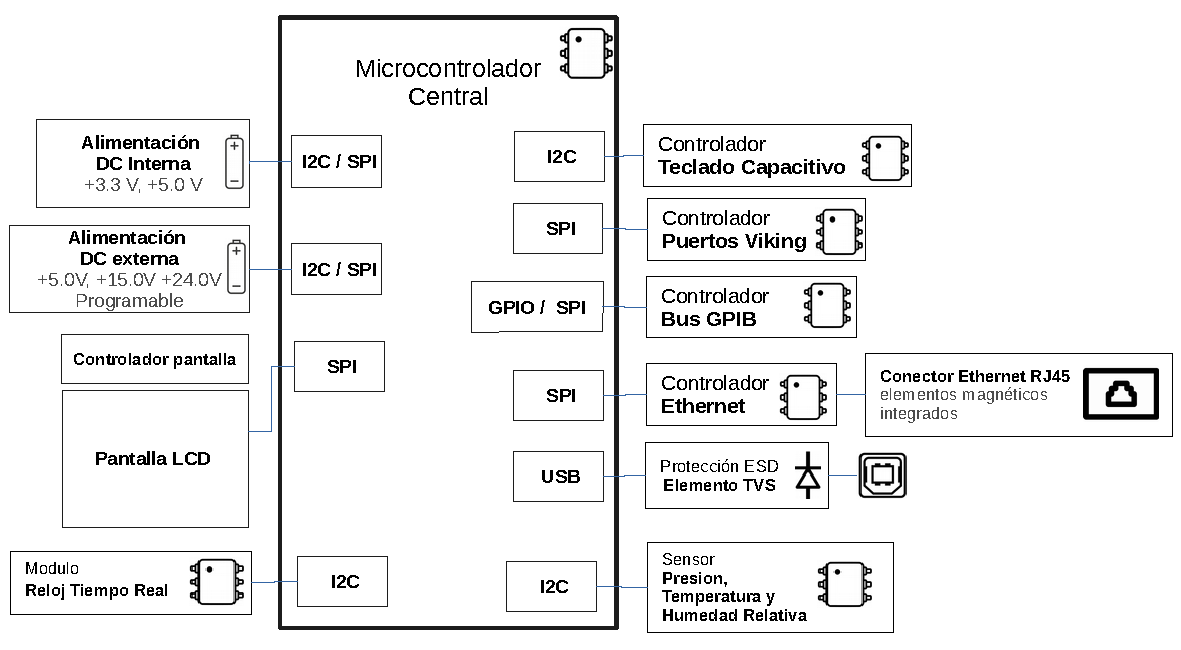
\includegraphics[width=16cm]{Cendit11713BloquesAntes.pdf} \\
		\end{center}

		\begin{center}
			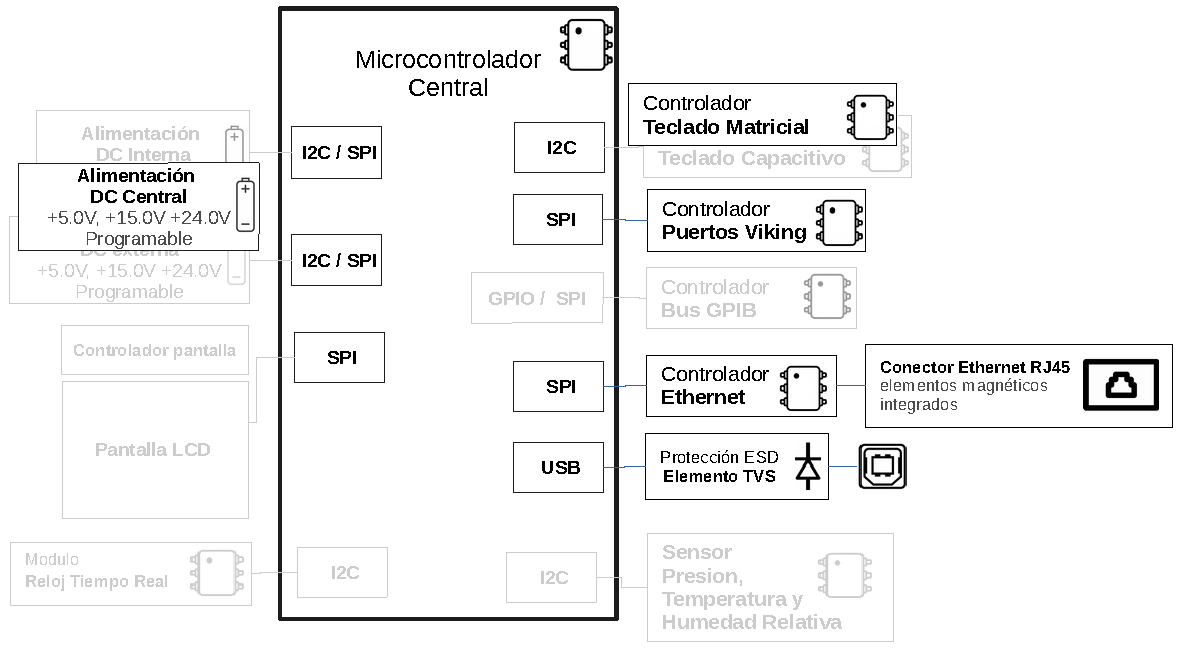
\includegraphics[width=16cm]{Cendit11713BloquesDespues.pdf}
		\end{center}	
	
	\subsection{Pautas}
	
	\begin{enumerate}
	
		\item Una solución de tipo “quick and dirty” para el dispositivo electrónico. Esta es la solución para la UCV. Se realizará una tarjeta madre PCB los más simple posible, tal vez empleando un integrado de tipo thru-hole (no de montaje superficial) en donde reside el micro central acompañado de varios conectores (tiras de pines – pin headers) en cada uno de sus puertos. En estas tiras de pines por medio de cable de cinta se conectará en uno un teclado matricial simple (de 4 x 4), en los otros se conectan las tarjetas expansoras, una de ellas con los transceptores para el bus GPIB.
		
		\item Una aplicación del mismo tipo, “quick and dirty”, únicamente con cuatro pantallas para cada proceso de medición, configuración y calibración para: medición de figura de ruido, medición de potencia de ruido, medición de ganancia, configuración. Esta aplicación es para la UCV. En principio no posee capacidad para corrección por medio de parámetros S de los dispositivos de conexión ni capacidad de simulación. Estas características se agregaran si hay tiempo y una vez completada las tarjetas PCB.
		
		\item Me preocupa el desarrollo del bus GPIB, en cuanto no he podido conseguir los IC transceivers de bus. Además, la documentación que he conseguido en superficial, a nivel de usuario, no detalla la capa de comunicaciones (señales + diagramas de tiempo.). La especificación de este bus IEEE-488 no se consigue de forma libre, hay que pagar por ella. En cambio, para el controlador LAN, en la página de Microchip abunda la información.
	
	\end{enumerate}
	
	\subsection{Cronograma inicial TEG}
	
		\begin{threeparttable}[!h]
			\centering
			\arrayrulecolor{gray}
			\setlength{\extrarowheight}{4pt}		
			\resizebox{\textwidth}{!}{
				\begin{tabular}{|c|l|l|l|l|l|l|l|l|l|l|l|l|l|l|l|l|l|l|l|l|l|l|l|l|l|l|l|l|}
					\hline 			
					\textbf{Semanas} & 1 & 2 & 3 & 4 & 5 & 6 & 7 & 8 & 9 & 10 & 11 & 12 & 13 & 14 & 15 & 16 & 17 & 18 & 19 & 20 & 21 & 22 & 23 & 24 & 25 & 26 & 27 & 28 \\
					\hline
					\textbf{Fase 1}
					& \fa & \fa & \fa & \fa & \fa & \fa & & & & & & & & & & & & & & & & & & & & & & \\			
					\hline			
					\textbf{Fase 2} & & & & & & & \fb & \fb & \fb & \fb & \fb & \fb & \fb & \fb & \fb & \fb & \fb & & & & & & & & & & & \\
					\hline
					\textbf{Fase 3} & & & & & & & & & & & & & & & & & & \fc & \fc & \fc & \fc & \fc & & & & & & \\	
					\hline		
					\textbf{Seminario} & & & & & & & & & & & & & & \sem & & & & & & & & & & & & & & \\
					\hline
					\textbf{Fase 4} & & & & & & & & & & & & & & & & & & & & & & & \fd & \fd & \fd & \fd &  & \\
					\hline
					\textbf{Fase 5} & & & & & & & & & & & & & & & & & & & & & & & & & & & \fe & \fe \\
					\hline	
				\end{tabular}
			}
			\begin{tablenotes}
				\item {\tiny Fecha de inicio: 6 de Marzo de 2017.} 
				\item {\tiny Jornada de 8 horas diarias, lunes a viernes, de 8:00 AM a 12:00 M y de 1:30 PM a 4:30 PM.}
			\end{tablenotes}
		\end{threeparttable}
	
	\subsection{Contabilidad horaria}
	
		\begin{figure}[h!]
			\centering
			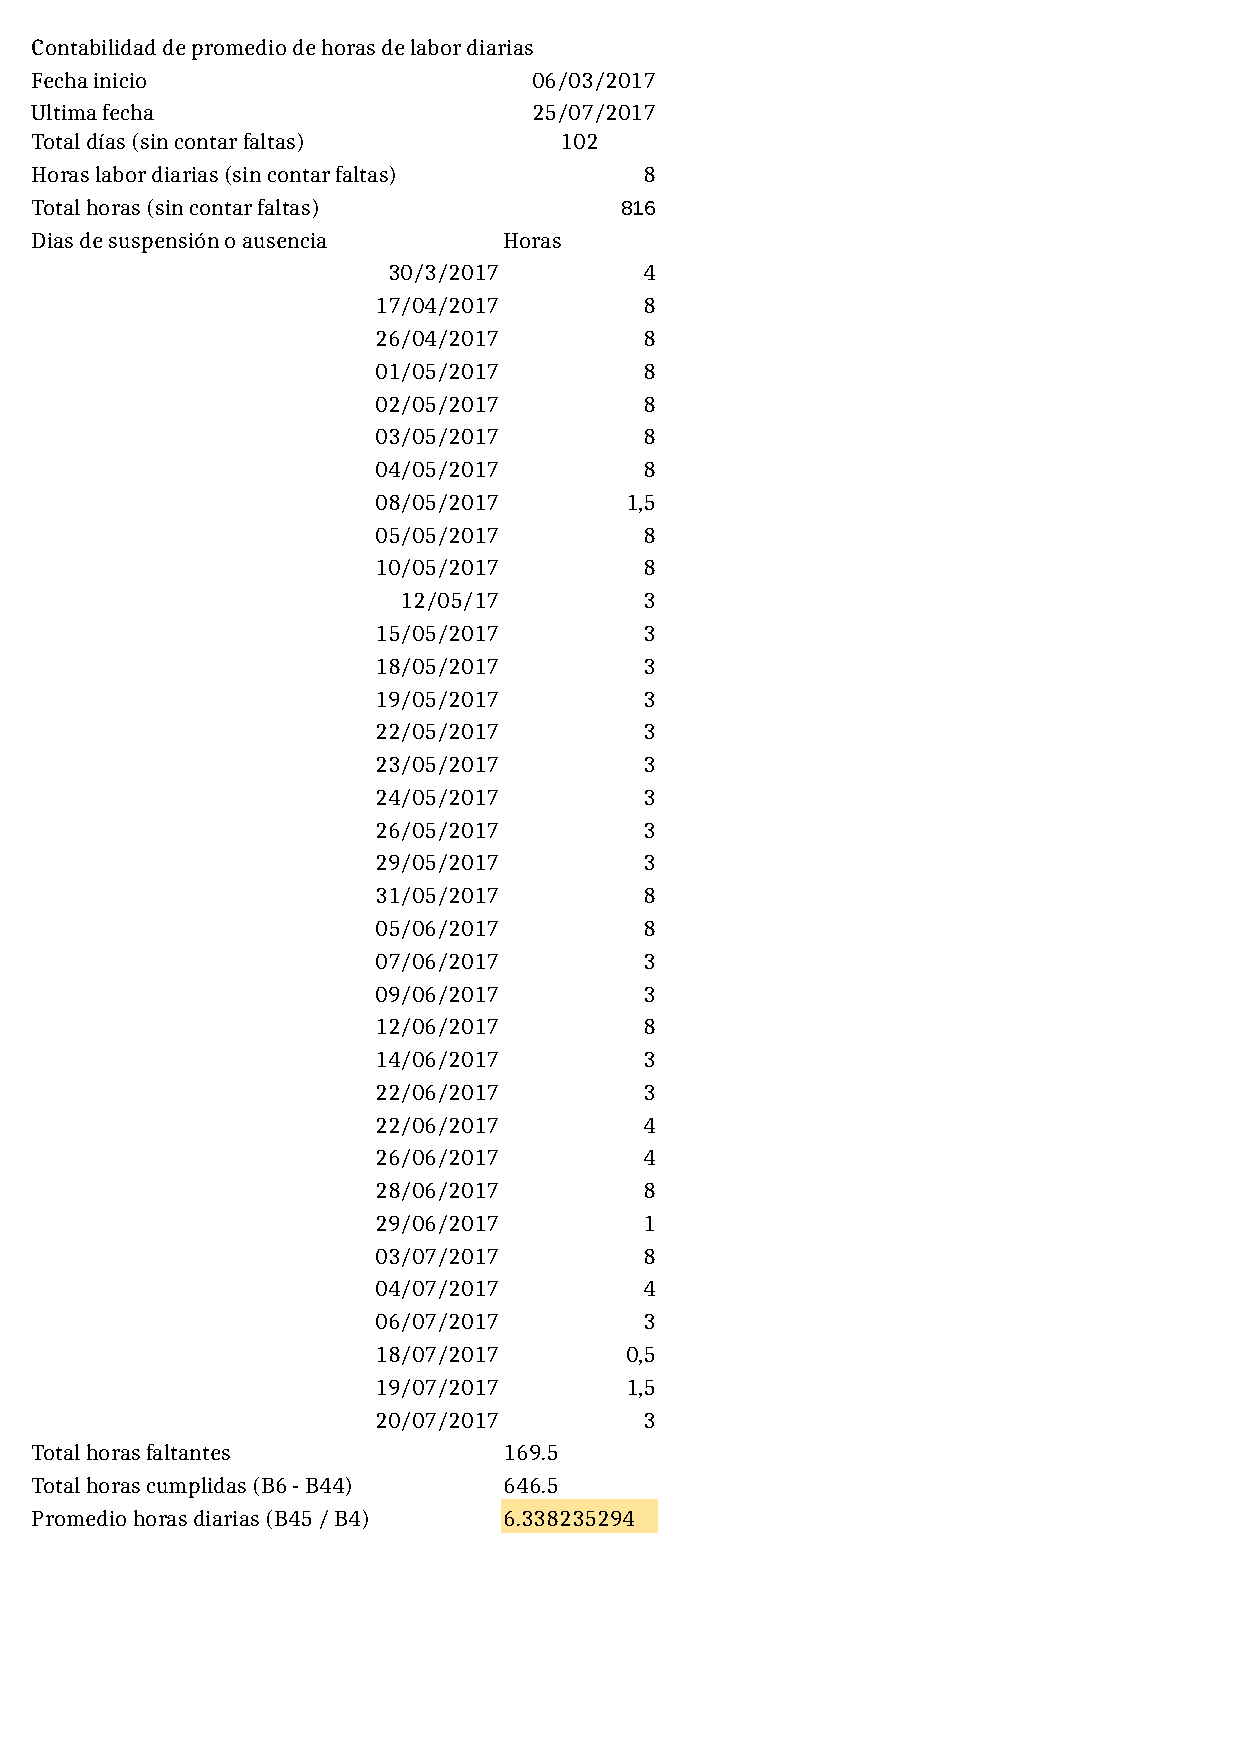
\includegraphics[width=10cm]{ContabilidadHorasPasantia.pdf}
		\end{figure}
	
		\begin{table}[h!]
		\resizebox{\linewidth}{!}{%
			\begin{tabular}{cllllc}
				\toprule
				\bfseries Item & \bfseries  Tarea & \bfseries  Entrada & \bfseries  Proceso & \bfseries  Salida & \bfseries  Semanas \\
				\midrule
				1 & Expansor puertos Viking & 
				\begin{tabular}{l}
					Materiales desarrollo PCB \\
					Circuitos integrados \\
					Aplicaciones EDA (KiCad, Eagle, Proteus)
				\end{tabular} &			
				\begin{tabular}{l}
					Diseño esquemáticos \\
					Revisión esquemáticos \\
					Selección de componentes \\
					Simulación \\
					Elaboración PCB \\
					Soldadura de componentes \\
					Depuración tarjeta individual \\
					Integración con tarjeta madre
				\end{tabular} &
				\begin{tabular}{l}
					Tarjeta en PCB				
				\end{tabular} &
				4 \\
				
				\midrule			
				1 & Expansor puertos Viking & 
				\begin{tabular}{l}
					Materiales desarrollo PCB \\
					Circuitos integrados \\
					Aplicaciones EDA (KiCad, Eagle, Proteus)
				\end{tabular} &			
				\begin{tabular}{l}
					Diseño esquemáticos \\
					Revisión esquemáticos \\
					Selección de componentes \\
					Simulación \\
					Elaboración PCB \\
					Soldadura de componentes \\
					Depuración tarjeta individual \\
					Integración con tarjeta madre
				\end{tabular} &
				\begin{tabular}{l}
					Tarjeta en PCB				
				\end{tabular} &
				4 \\	
				
				\midrule			
				2 & Tarjeta interfaz usuario & 
				\begin{tabular}{l}
					Materiales desarrollo PCB \\
					Elementos mecánicos (botones, cables, tornillos) \\
					Aplicaciones EDA (KiCad, Eagle) \\
				\end{tabular} &			
				\begin{tabular}{l}
					Diseño esquemáticos \\
					Revisión esquemáticos \\
					Selección de componentes \\
					Elaboración PCB \\
					Soldadura de componentes \\
					Pruebas de tarjeta individual \\
					Integración con tarjeta madre \\
				\end{tabular} &
				\begin{tabular}{l}
					Tarjeta de interfaz de usuario \\
					Teclado matricial.		
				\end{tabular} &
				1 \\			
				
				\midrule			
				3 & Firmware del dispositivo & 
				\begin{tabular}{l}
					Computador PC \\
					Tarjeta madre prototipo \\
					Aplicaciones IDE (MPLAB-X) \\
					Aplicaciones simulación electrónica (Proteus) \\
				\end{tabular} &			
				\begin{tabular}{l}
					Identificación de componentes \\
					Modelado de componentes \\
					Codificación \\
					Carga de firmware \\
					Pruebas aisladas \\
					Pruebas con periféricos individuales \\
					Integración \\
					Pruebas finales \\
				\end{tabular} &
				\begin{tabular}{l}
					Firmware controlador del dispositivo Cendit11713
				\end{tabular} &
				6 \\			
				
				\midrule			
				4 & Tarjeta madre & 
				\begin{tabular}{l}
					Materiales desarrollo PCB \\
					Circuitos integrados \\
					Elementos pasivos (resistores, capacitores) \\
					Elementos mecánicos (conectores de puertos, retenedores, tornillos) \\
					Carcasa metálica \\
					Aplicaciones EDA (KiCad, Eagle) 
				\end{tabular} &			
				\begin{tabular}{l}
					Diseño de esquemáticos \\
					Revisión de esquemáticos \\
					Selección de componentes \\
					Simulación \\
					Elaboración PCB \\
					Soldadura de componentes \\
					Carga de firmware \\
					Pruebas de tarjeta individual \\
					Integración con periféricos
				\end{tabular} &
				\begin{tabular}{l}
					Tarjeta madre en PCB		
				\end{tabular} &
				4 \\			
				
				\midrule			
				5 & Tarjeta alimentación DC
				& 
				\begin{tabular}{l}
					Materiales desarrollo PCB \\
					Circuitos integrados \\
					Elementos pasivos (resistores, capacitores) \\
					Elementos mecánicos (conectores de puertos, retenedores, tornillos) \\
					Cables \\
					Aplicaciones EDA (KiCad, Eagle, Spice) 
				\end{tabular} &			
				\begin{tabular}{l}
					Diseño de esquemáticos \\
					Revisión de esquemáticos \\
					Selección de componentes \\
					Simulación \\
					Elaboración PCB \\
					Soldadura de componentes \\
					Pruebas de tarjeta individual 
				\end{tabular} &
				\begin{tabular}{l}
					Tarjeta en PCB	
				\end{tabular} &
				5 \\			
				
				\midrule				
				6 & Aplicación SGMFR & 
				\begin{tabular}{l}
					Computador PC \\
					Acceso a internet \\
					Bibliografía \\
					Aplicaciones IDE (JIDEA) \\
					JDK (librerías Java) \\
					Librerías comunicaciones con instrumentos 
				\end{tabular} &			
				\begin{tabular}{l}
					Identificación de componentes \\
					Modelado de componentes \\
					Codificación \\
					Pruebas \\
					Integración 
				\end{tabular} &
				\begin{tabular}{l}
					Aplicación funcional e instalador
				\end{tabular} &
				8 \\		
				
				\midrule			
				7 & Documentación
				&
				\begin{tabular}{l}
					Computador PC \\
					Acceso a internet \\
					Bibliografía \\
					Distribución de \LaTeX \\
					Editor de \LaTeX \\
				\end{tabular} &			
				\begin{tabular}{l}
					Recopilación de documentos \\
					Lectura \\
					Toma de notas \\
					Organización de notas \\
					Escritura de libro TEG \\
					Escritura de informes
				\end{tabular} &
				\begin{tabular}{l}
					Libro de TEG \\
					Informe técnico \\
					Instrucciones de trabajo 
				\end{tabular} &
				8 \\							
				\bottomrule
			\end{tabular}%
		}
		\caption{Descripción de actividades del cuadro \ref{Tab:CronogramaActividadesInicial}}
	\end{table}
	
\end{document}